\graphicspath{{introduction/fig/}}

\chapter{Introduction}
\label{chap:introduction}

\section{Background}
In South Africa, millions of commuters use taxis frequently and depend on them for all of their mobility needs \cite{depttransport2023}. The South African government has recognised the impact of taxi emissions on air quality and has taken steps to address the issue. In 2006, the government gazetted regulations that required taxi operators to convert their vehicles to run on cleaner fuels, such as liquefied petroleum gas (LPG), compressed natural gas (CNG), or diesel with lower sulphur content\cite{2007Comparison}. 

\begin{figure}[!htb]
	\minipage{0.32\textwidth}%
	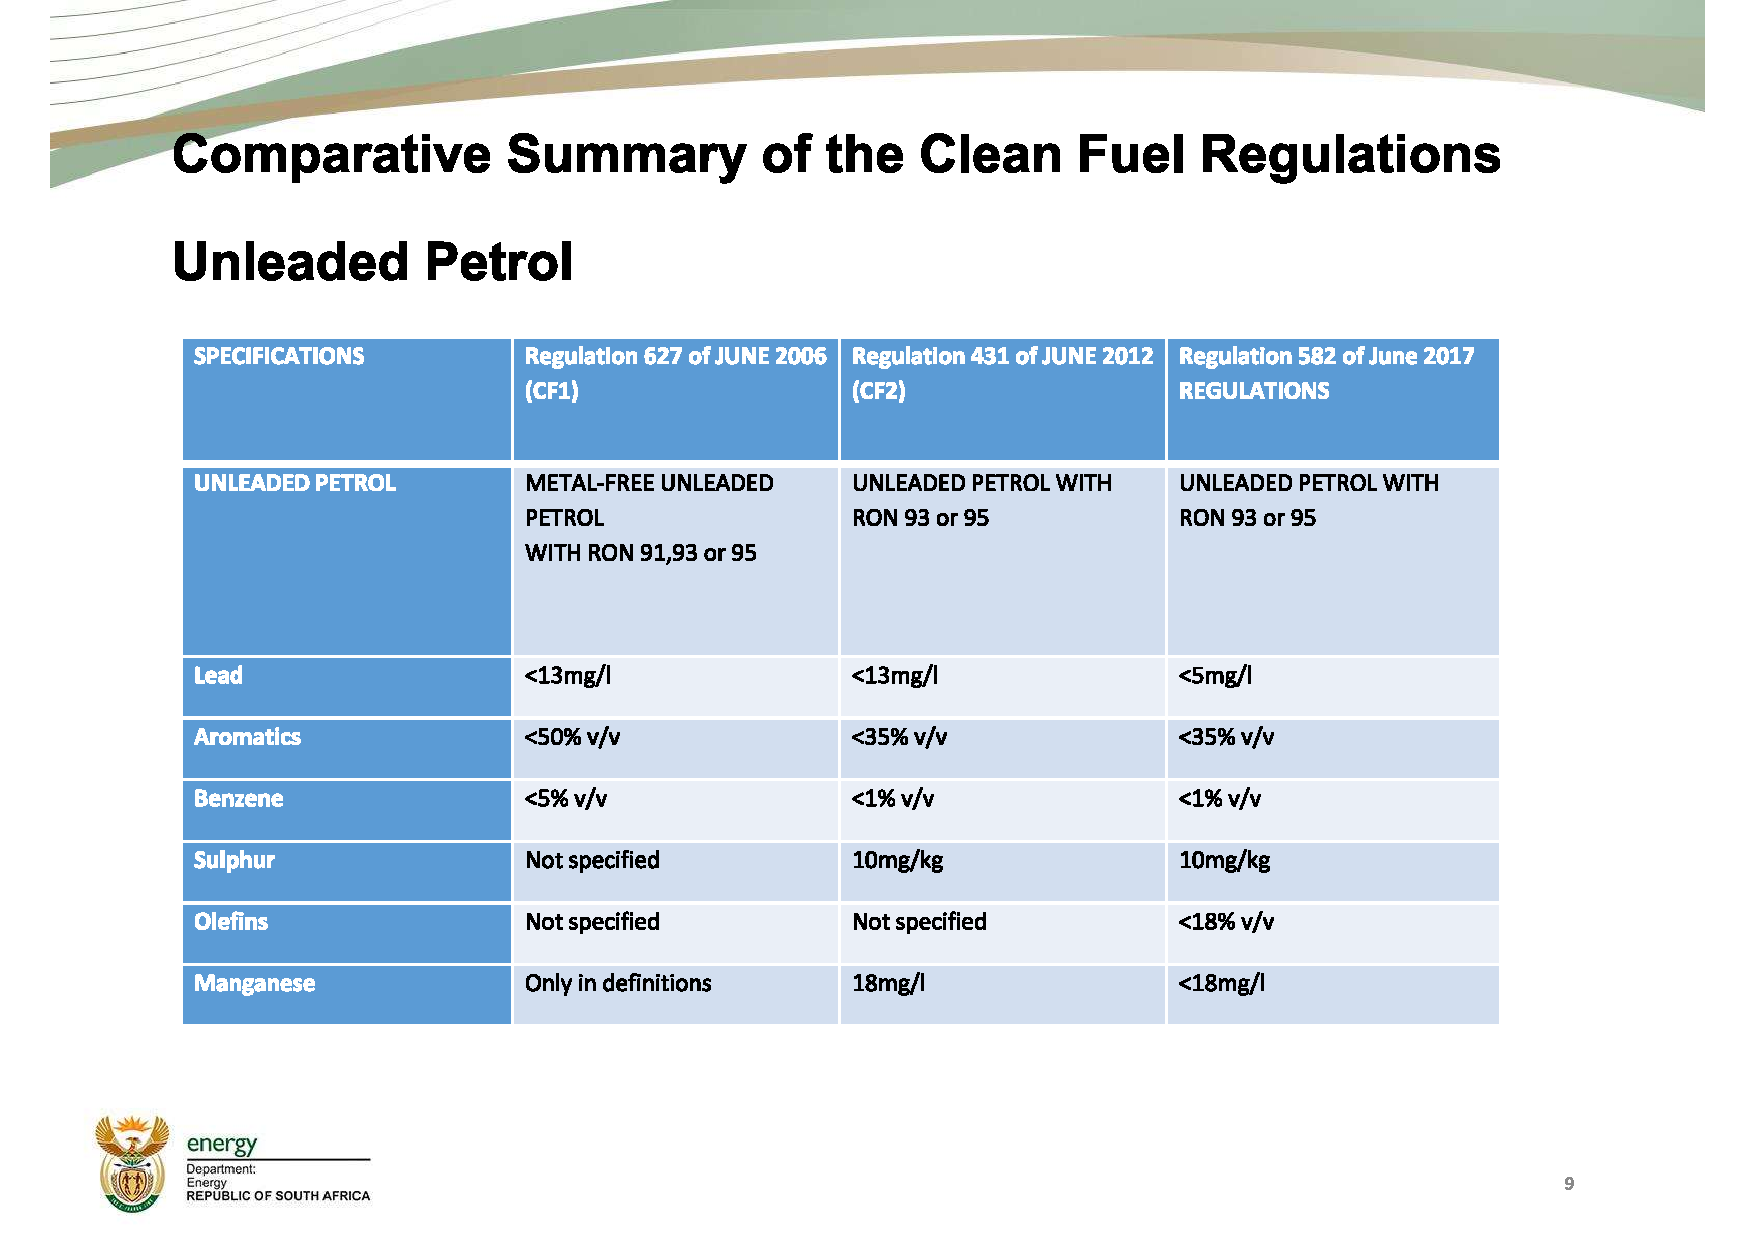
\includegraphics[width=\linewidth]{introduction/fig/page1Comp.pdf}
	\caption{Unleaded\cite{2007Comparison}}\label{fig:fig1}
	\endminipage\hfill
	\minipage{0.32\textwidth}%
	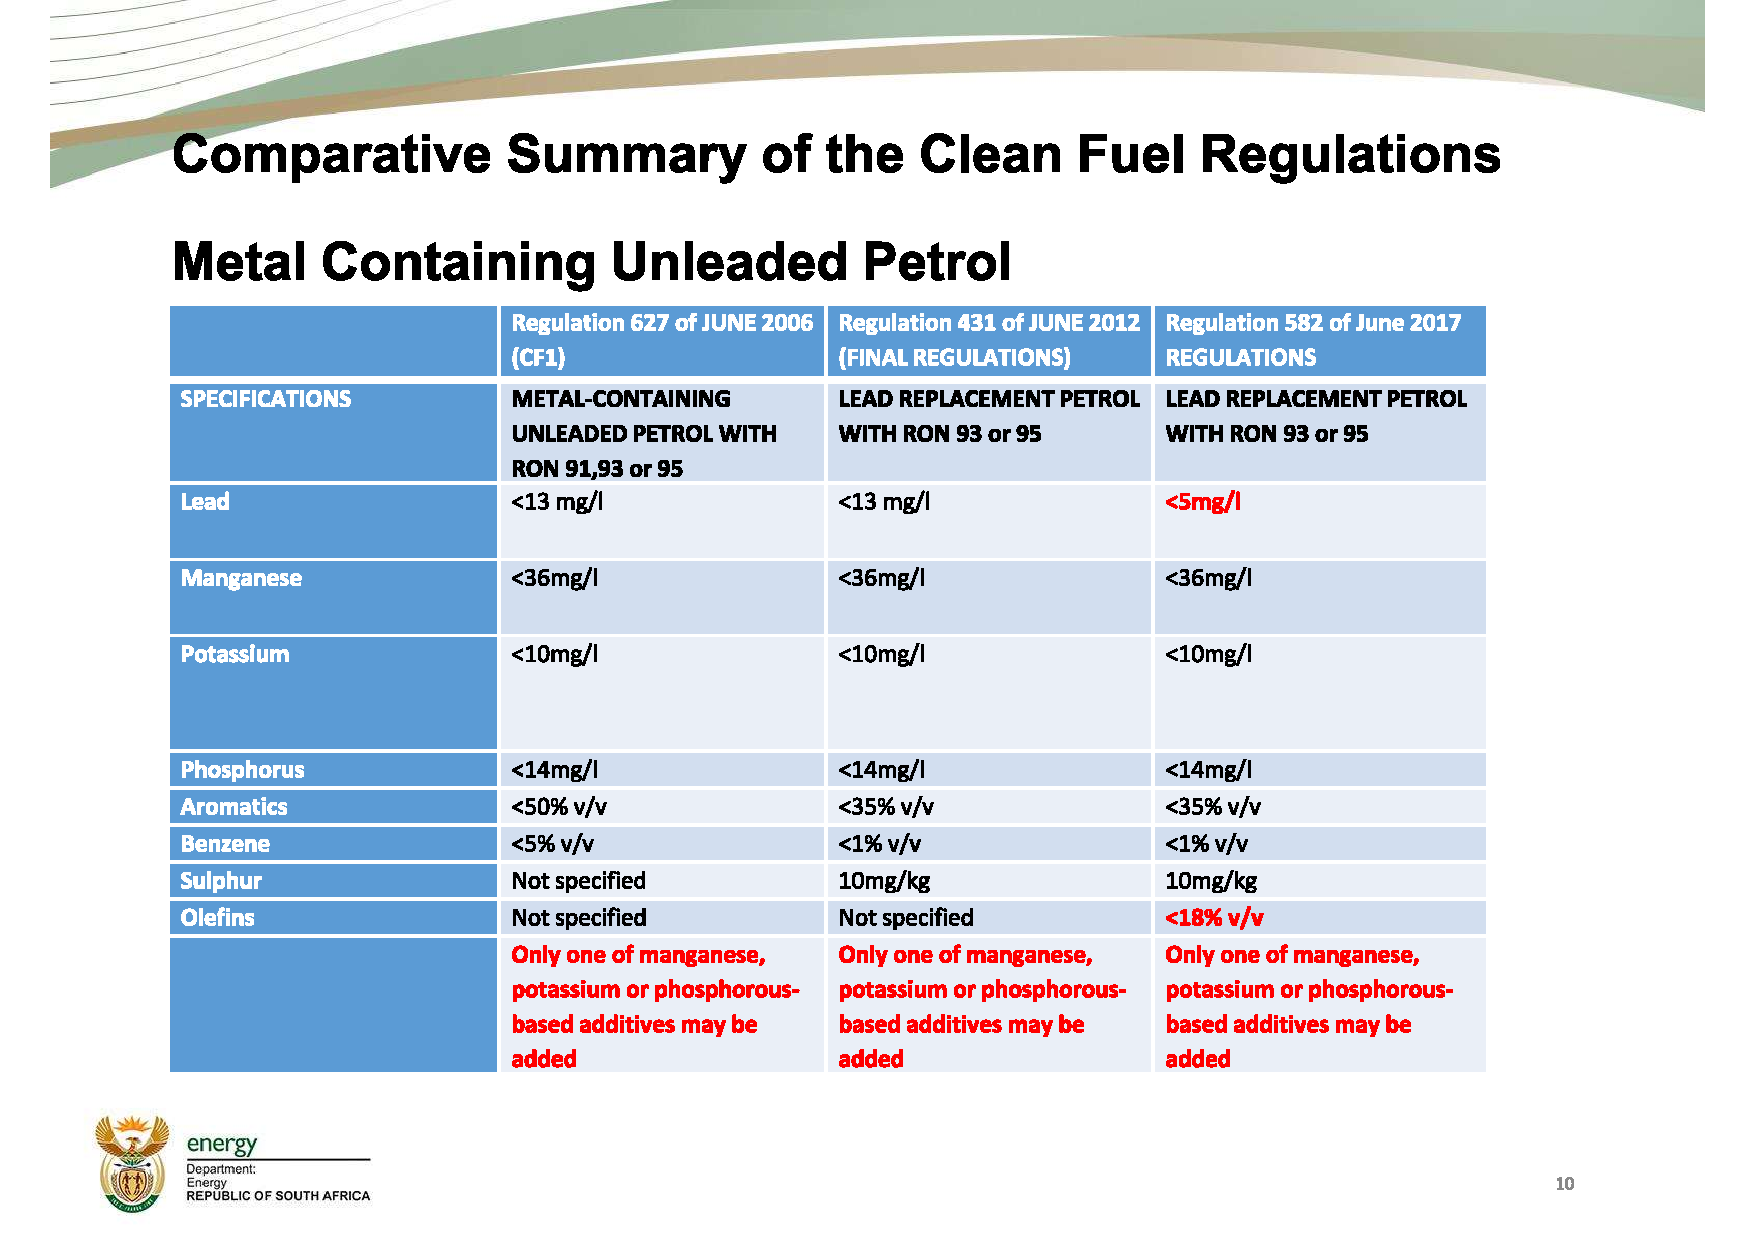
\includegraphics[width=\linewidth]{introduction/fig/page2Comp.pdf}
	\caption{Metal+ Unleaded\cite{2007Comparison}}\label{fig:fig2}
	\endminipage\hfill
	\minipage{0.32\textwidth}%
	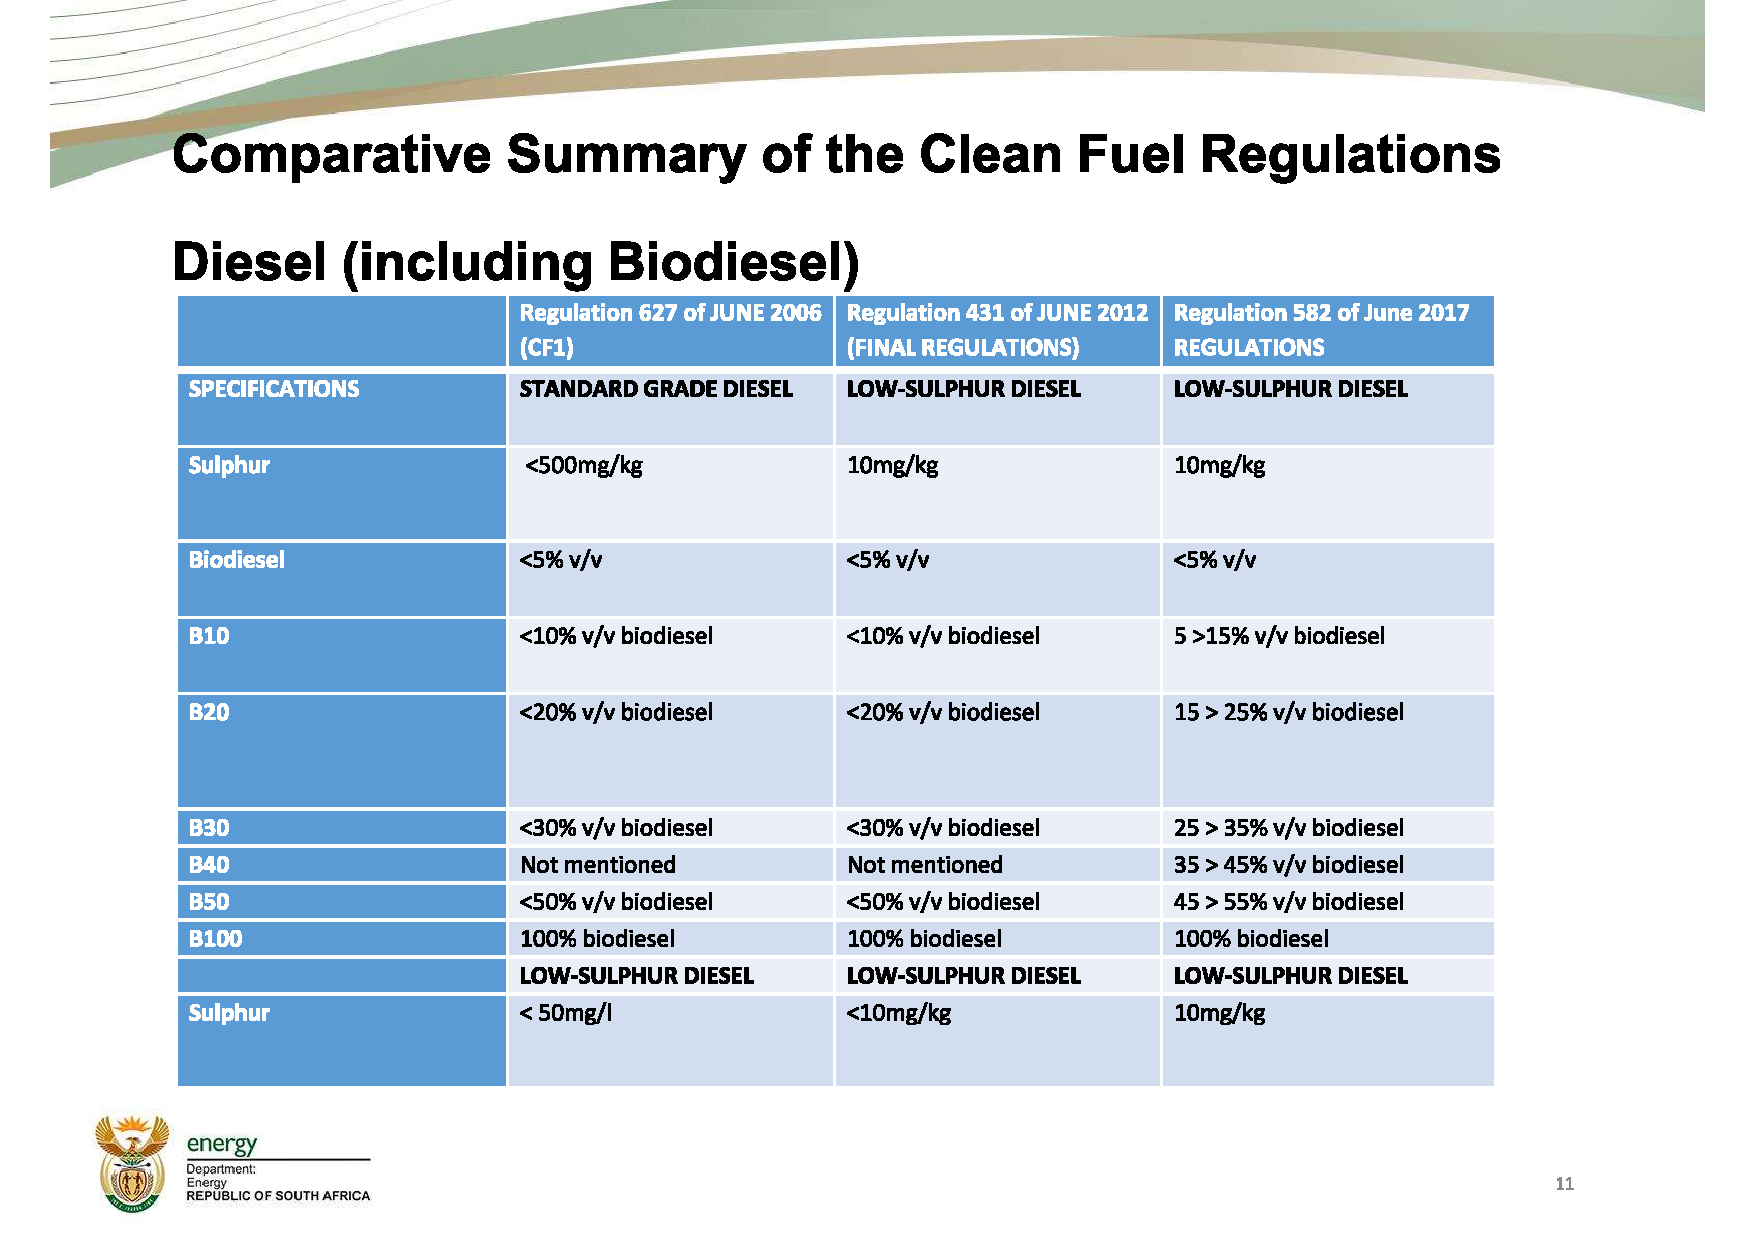
\includegraphics[width=\linewidth]{introduction/fig/page3Comp.pdf}
	\caption{Diesel\cite{2007Comparison}}\label{fig:fig3}
	\endminipage
	%\text{Charts provided by \cite{2007Comparison}}
\end{figure}

\noindent
As seen in Figures \ref{fig:fig1}, \ref{fig:fig2} and \ref{fig:fig3}, South Africa's regulations on cleaner fuels are updated every five to six years. Cleaner fuels produce less greenhouse emissions. The implementation of these regulations has been slow and often poorly regulated \cite{newcleanfuelstandards}, resulting in continued poor air quality in many areas.

\noindent
The main sources of air pollution in South Africa are industrial activities, power generation, vehicle emissions, biomass burning, and domestic fuel use \cite{Bylaws2023}. Among these sources, vehicle emissions are particularly relevant for taxi commuters, who are exposed to high levels of pollutants such as particulate matter (PM), nitrogen oxides (NOx), carbon monoxide (CO), and volatile organic compounds (VOCs) \cite{Venter2018}. These pollutants can have adverse effects on respiratory, cardiovascular, neurological, and immune systems, as well as increase the risk of cancer and premature death \cite{WHO2016}.

%Instead of using expensive and inconvenient formal public transportation like buses and trains, they offer an accessible and affordable substitute.

%{\color{red} \huge Need to rewrite}
\section{Problem Statement}
Despite the popularity and importance of taxis in South Africa, there is a lack of research on the air quality inside these vehicles and at taxi ranks. 
Air quality is a crucial factor for human health and well-being, especially for commuters who spend long hours in taxis, and potentially exposed to various pollutants.
Moreover, taxi emissions contribute to the overall air pollution in crowded spaces (in this case taxi ranks), which affects the environment and the quality of life of the passers-by. The closest studies to this one are concerning single cab taxis\cite{insidetaxismall}, road-based pollution\cite{taxiNetwork} and general pollution\cite{Environmentalimpact}.
There is a need for a study on the air quality in taxis and taxi ranks and its impacts on human health and the environment, this report aims to provide a means to that end.

\section{Objectives}
The objectives of the study are as follows:
\begin{enumerate}
	\item To perform a literature study on the typical  airborne contaminants with which to evaluate air quality and their impacts on health. .
%	\item Identify the primary sources of air pollution in taxi ranks and within taxis and evaluate the impact of environmental factors, such as traffic congestion and weather conditions(optional- time limited).
	\item To perform a study to determine the ways in which to monitor those contaminants with electronic sensors. 
%	\item To evaluate the effectiveness of current measures in place to reduce air pollution from taxis, such as emission standards and regulations.
	\item To develop an electronic solution to facilitate the distributed and mobile measurement of air quality in minibus taxis and around taxi ranks. 
          \begin{enumerate}
	           \item Develop a stationary base station to measure air quality at the ranks and to receive and convey (as gateway) air quality measured inside minibus taxis. 
              \item Develop a mobile air quality sensor that autonomously transfer measure air quality data to the base station when it comes within radio communications range of the gateway.
	       \end{enumerate} 
	%\item Develop software/firmware that integrates the hardware.
%	\item Propose potential strategies to mitigate the impact of  from taxis on public health and the environment such as implementing new technologies.
\end{enumerate}


%\section{Summary of Work}??


\section{Scope}
The scope of the project encompasses only the following:

\begin{itemize}
	\item Design of base station and satellite module
	\item Design of communication network for satellite module and base station as well as data storage and backup
	%\item Deployment of sensor and network
%	\item Analysis of data gathered
	\item Hardware development
	\item Software development
	\item Test of Hardware and Software elements
\end{itemize}

\section{Report Overview}%Roadmap

in this thesis report, Chapter 1 presents the summary of the scope and reasoning of  the project and the problems it addresses. In Chapter 2, literature is provided to give an understanding of why the solution is needed as well as other examples of similar solutions or research. Chapter 3 provides an overview of the design step of the project and also introduces the hardware used and the considerations. Chapter 4 delves deeper into the hardware that was chosen and its features as well as how it is implemented in the project, it also provides a view of the coding or firmware involved in bringing it to fruition. Chapter 5 contains the results of the solution and shows it in action. Chapter 6 contains the summary, conclusion and future work and recommendations.






